\documentclass[12pt,a4paper]{article}
\usepackage[utf8]{inputenc}
\usepackage[T1]{fontenc}
\usepackage{graphicx}
\usepackage{geometry}
\usepackage{amsmath}
\usepackage{array} %Per tabella
% \usepackage{caption}
% \captionsetup[table]{labelformat=empty} %per evitare scritta Table1,Table2, ecc

% https://latexeditor.lagrida.com/ per simboli latex
% simboli $\mathcal{O}(n)$, $\Theta(...)$, $\Omega(n)$

\graphicspath{ {./plots/} }
\geometry{ top=40mm, bottom=40mm, left=30mm, right=30mm} 

\title{\textbf{Implementation and Analysis of BST, AVL and RBT Data Structures}}
\author{Sebastiano Babich (172249) - Leonardo Mazzon (172587) \\- Damiano Netto (171948)}
\date{University of Udine, Academic Year 2025 - 2026}

\begin{document}
	\maketitle
	\tableofcontents
	\newpage

	\section{Abstract}

		The goal of the project was to implement and compare some of the data structures studied in the “Algorithms and Data Structures” course at the University of Udine, specifically standard and self-balancing binary search trees. The project focused in particular on the time complexity involved in inserting and deleting data within these structures. We also decided to analyze the heights reached by the trees during the various operations and to count the number of rotations performed on each tree.

	\section{Introduction}

		Search trees are among the most widely used data structures, since they enable high performance in both searching, inserting and deleting data. Specifically, the trees used in our project are binary: each node has at most two children, which can be other nodes or pointers to NULL.The resulting tree is acyclic, and one of its most important characteristics is its height that is defined as the maximum number of nodes on the path from the root to any leaf.
		\\[10pt]
		

	\section{Theorical Background}
		In all of the data structures which implements search trees, height is a fundamental property: keeping its value as small as possible helps ensure efficient operations thanks to more efficient search, insertion and deletion operations.
		\\[10pt]
		Trees can be divided into two categories based on how they manage their height: \textbf{binary search trees} and \textbf{balanced binary trees}. Standard binary search trees do not actively control their height, while balanced binary trees use specific rules and rotation operations to keep the height as small as possible.
		\\[10pt]
		Trees belonging to the second category are designed to maintain a height close to the order of $\log_2(n)$, where $n$ is the number of nodes inserted into the tree.
		\\[10pt]
		In this project, we studied three types of trees, two of which implement self-balancing techniques.

		\subsection{Binary Search Tree (BST)}

			Binary search trees do not impose any restrictions on their height. Their main purpose is to provide efficient search, insertion and deletion operations maintaining an ordered structure of the stored elements. However, since they do not include any mechanism to control their height, the tree can become unbalanced depending on the order in which nodes are inserted. As the number of nodes increases, this can lead to a significant degradation in performance, especially in the worst-case scenario.


			\begin{table}[h]
				\centering
				\begin{tabular}{c|c|c}
				\hline
				\textbf{Operation} & \textbf{Average Case} & \textbf{Worst Case} \\
					\hline
						Search of a Node & $\mathcal{O}(\log n)$ & $\mathcal{O}(n)$ \\
						Insertion of a Node & $\mathcal{O}(\log n)$ & $\mathcal{O}(n)$ \\
						Deletion of a Node & $\mathcal{O}(\log n)$ & $\mathcal{O}(n)$ \\
					\hline
				\end{tabular}
				\caption{Time complexity in BST operations}
			\end{table}



		\subsection{Adelson-Velsky Landis Tree (AVL)}

			AVL trees are a data structure that implements self balancing binary search trees. The search operation in the tree exactly mirrors the search in BST. Insertion initially uses the BST insertion method, with the difference that a self balancing operation is performed afterward.
			\\[10pt]
			Specifically, this operation aims to identify imbalances in the tree by comparing the heights of two child nodes. Specifically, the goal is to minimize the total height of the tree, so that search operations remain as close as possible to logarithmic complexity.
			\\[10pt]
			
			\begin{table}[h]
				\centering
				\begin{tabular}{c|c|c}
				\hline
				\textbf{Operation} & \textbf{Average Case} & \textbf{Worst Case} \\
					\hline
						Search of a Node & $\mathcal{O}(\log n)$ & $\mathcal{O}(\log n)$ \\
						Insertion of a Node & $\mathcal{O}(\log n)$ & $\mathcal{O}(\log n)$ \\
						Deletion of a Node & $\mathcal{O}(\log n)$ & $\mathcal{O}(\log n)$ \\
					\hline
				\end{tabular}
				\caption{Time complexity in AVL operations}
			\end{table}
		\subsection{Red Black Tree (RBT)}
			...


			\begin{table}[h]
				\centering
				\begin{tabular}{c|c|c}
				\hline
				\textbf{Operation} & \textbf{Average Case} & \textbf{Worst Case} \\
					\hline
						Search of a Node & $\mathcal{O}(\log n)$ & $\mathcal{O}(\log n)$ \\
						Insertion of a Node & $\mathcal{O}(\log n)$ & $\mathcal{O}(\log n)$ \\
						Deletion of a Node & $\mathcal{O}(\log n)$ & $\mathcal{O}(\log n)$ \\
					\hline
				\end{tabular}
				\caption{Time complexity in RBT operations}
			\end{table}

	\section{Implementation}
		The data structures (BST, AVL and RBT) were implemented as separate modules in the project, with similar interfaces for insertion, deletion, and search. Each tree maintains additional information useful for analysis, such as current height and number of rotations. Balancing operations were separated into dedicated functions within each type of tree to comply with the rules imposed by the data structure used.

	\section{Test Cases Setup}
		
		Per l'impostazione dei casi di test abbiamo inizialmente pensato a quali potessero essere 
		For the test cases, we have divided the code into three separate files:

		\begin{itemize}
			\item \textit{setup\_test.py}: 
			\item \textit{test\_insertion.py}: 
			\item \textit{test\_rotations.py}: 
		\end{itemize}

	\section{Results and Discussion}
		\subsection{Test sugli inserimenti}
			\begin{figure}[h]
				\centering
				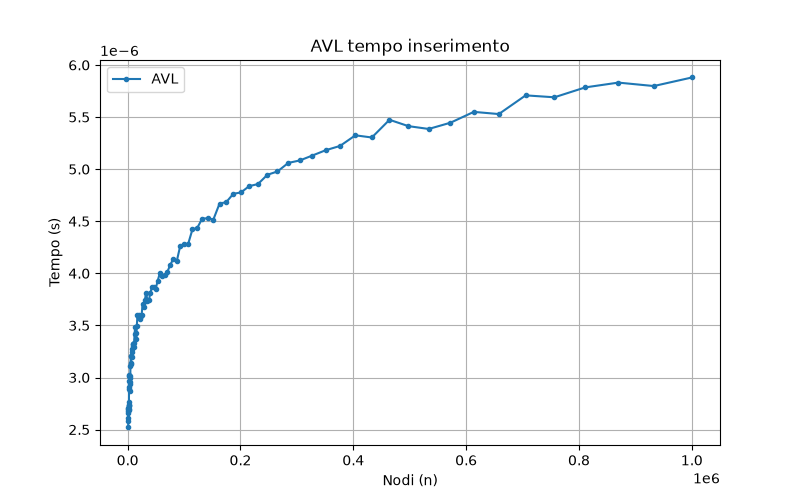
\includegraphics[width=0.8\textwidth]{AVL_14-01-33-plot} 
				\caption{Test eseguito}
			\end{figure}

		\subsection{Test sul numero di rotazioni}
			

		\subsection{Test sull'altezza dell'albero}

	\section{Conclusion}

		To conclude this project, we compared all the data structures we analyzed and drew conclusions regarding the ideal use cases for each type of tree.

		\subsection{Confrontro tra le strutture dati analizzate}
			
		\subsection{Final Remarks}
			The comparison demonstrates that the additional complexity required to implementing self-balancing trees is justified by the significant long-term gains in efficiency and robustness offered by these data structures.
\end{document}